% !TeX encoding = UTF-8
% !TeX spellcheck = es_ES

\documentclass[25pt,a0paper,portrait]{tikzposter}
\usepackage[spanish]{babel}
\usepackage[utf8]{inputenc}
%\usepackage[T1]{fontenc}
%\usepackage{lmodern}
\usepackage[super]{nth}
\usepackage{graphicx}
\usepackage[affil-it]{authblk}
% \usepackage{lmodern}
\usepackage{etoolbox}
\usepackage{amsmath}
\usepackage{amssymb}
\usepackage{mathtools}
\renewcommand\Authfont{\LARGE}
\renewcommand\Affilfont{\Large\itshape}

\newlength\htblockbox
\newcommand{\mtblock}[3]{%
\block{#2}{%
\setlength{\htblockbox}{#1}%
\parbox[t][\htblockbox][c]{\linewidth}{#3}}}

\usetheme{Simple}
%\usetitlestyle{verticalShading}


\title{\parbox{\linewidth}{\centering drexml: una herramienta para el descubrimiento de dianas terapéuticas en Enfermedades Raras}}

\author[1,2]{\large Marina Esteban-Medina}
\author[1,2]{\large V\'ictor Manuel de la Oliva Roque}
\author[3,4,5,6]{\large Sara Herr\'aiz-Gil}
\author[7,1]{\large Mar\'ia Pe\~na-Chilet}
\author[1,2,8,9]{\large Joaqu\'in Dopazo}
\author[1,2,8]{\large Carlos Loucera}

\affil[1]{%
\large Platform for Computational Medicine, Andalusian Public Foundation Progress and Health-FPS, Seville, Spain}

\affil[2]{%
\large Computational Systems Medicine, Institute of Biomedicine of Seville (IBIS), Hospital Virgen del Roc\'io, Seville, Spain}

\affil[3]{%
\large Centro de Investigaci\'on Biom\'edica en Red de Enfermedades Raras (CIBERER-ISCIII), U714, Madrid, Spain}

\affil[4]{%
\large Departamento de Bioingenier\'ia, Universidad Carlos III de Madrid (UC3M), Madrid, Spain}

\affil[5]{%
\large Regenerative Medicine and Tissue Engineering Group, Instituto de Investigaci\'on Sanitaria-Fundaci\'on Jim\'enez D\'iaz University Hospital (IIS-FJD), Madrid, Spain}

\affil[6]{%
\large Epithelial Biomedicine Division, Centro de Investigaciones Energ\'eticas, Medioambientales y Tecnol\'ogicas (CIEMAT), Madrid, Spain}

\affil[7]{%
\large Platform of Big Data, AI and Biostatistics. Health Research Institute La Fe (IISLAFE). Valencia. Spain
}

\affil[8]{%
\large Centro de Investigaci\'on Biom\'edica en Red de Enfermedades Raras (CIBERER-ISCIII), U715, Seville, Spain}

\affil[9]{%
\large FPS/ELIXIR-es, Hospital Virgen del Roc\'io, Seville, Spain}

\institute{\Large{\bf\textsc{XVII Reunión anual CIBERER (2024)}}}

%Make title customizer
\makeatletter
\def\maketitle{\AB@maketitle}
\makeatother

%% Optional title graphic
%\titlegraphic{\includegraphics[width=7cm]{IMG_1934}}
%% Uncomment to switch off tikzposter footer
\tikzposterlatexaffectionproofoff

\begin{document}
\maketitle[width=\linewidth,titletotopverticalspace=-0.05cm]

\block{Introducción}{
    \textsc{\textbf{DREXML}} es una herramienta de \textbf{software libre} que utiliza aprendizaje automático para \textbf{identificar nuevos usos para medicamentos existentes}. Se ha validado con éxito en dos enfermedades raras: Anemia de Fanconi, Melanoma Familiar,  COVID-19 y Retinitis Pigmentosa. El modelo identifica dianas terapéuticas para enfermedades específicas mediante el empleo de \textbf{aprendizaje automático y modelado mecanicista de la transducción de señale}s. En el caso de la Anemia de Fanconi, el modelo predice con éxito fármacos reutilizados previamente validados, mientras que en el caso del melanoma familiar, identifica un conjunto prometedor de fármacos para futuras investigaciones.
}

% \note[rotate=8, connection, width = 7cm,
% % roundedcorners=15, targetoffsetx=2cm
% ]{Oh wait! A note!}

\begin{columns}

    \column{0.33}
        \block{Mapa de la enfermedad}{
            \begin{itemize}
            \item Genes en Orphanet, DisGeNet, \dots?
            \item Control Vs Case?
            \item Pathways?
            \end{itemize}
        }

    \column{0.33}
        \block{Transducción de la Señal}{
            \[
                S_{n} = v_{n} \left(1 - \prod_{s_{a} \in A} \left( 1 - s_{a} \right) \right) \prod_{s_{i} \in I} \left( 1- s_{i} \right)
            \]
        }

    \column{0.34}
        \block{Contextualiza dianas}{
            \[
                \phi_i^k = \frac{1}{K!} \sum_{S \subseteq F \backslash\{i\}} \frac{|S|!(n_{circuits}-|S|-1)!}{n_{circuits}!} [f_x(S \cup \{i\}) - f_x(S)]   
            \]
        }

\end{columns}

\begin{columns}
    \column{0.33}
        \block{Construyendo puentes}{%

            Conectando \textbf{Diana - Enfermedad}. \\

            Usando \textbf{trasncriptómica pública} de \textbf{sanos}. \\

        }

        \block{Software y Publicación}{%
        \begin{tikzfigure}
            \includegraphics[width=0.25\linewidth]{./fig/drexml_pip.pdf} \hspace*{4cm}
            \includegraphics[width=0.25\linewidth]{./fig/drexml_doi.pdf}
        \end{tikzfigure}
        }

    \column{0.67}
        \block{Inferir el Impacto de las Dianas sobre el Mapa Mecanicista de la Enfermedad}{%
            \begin{tikzfigure}
            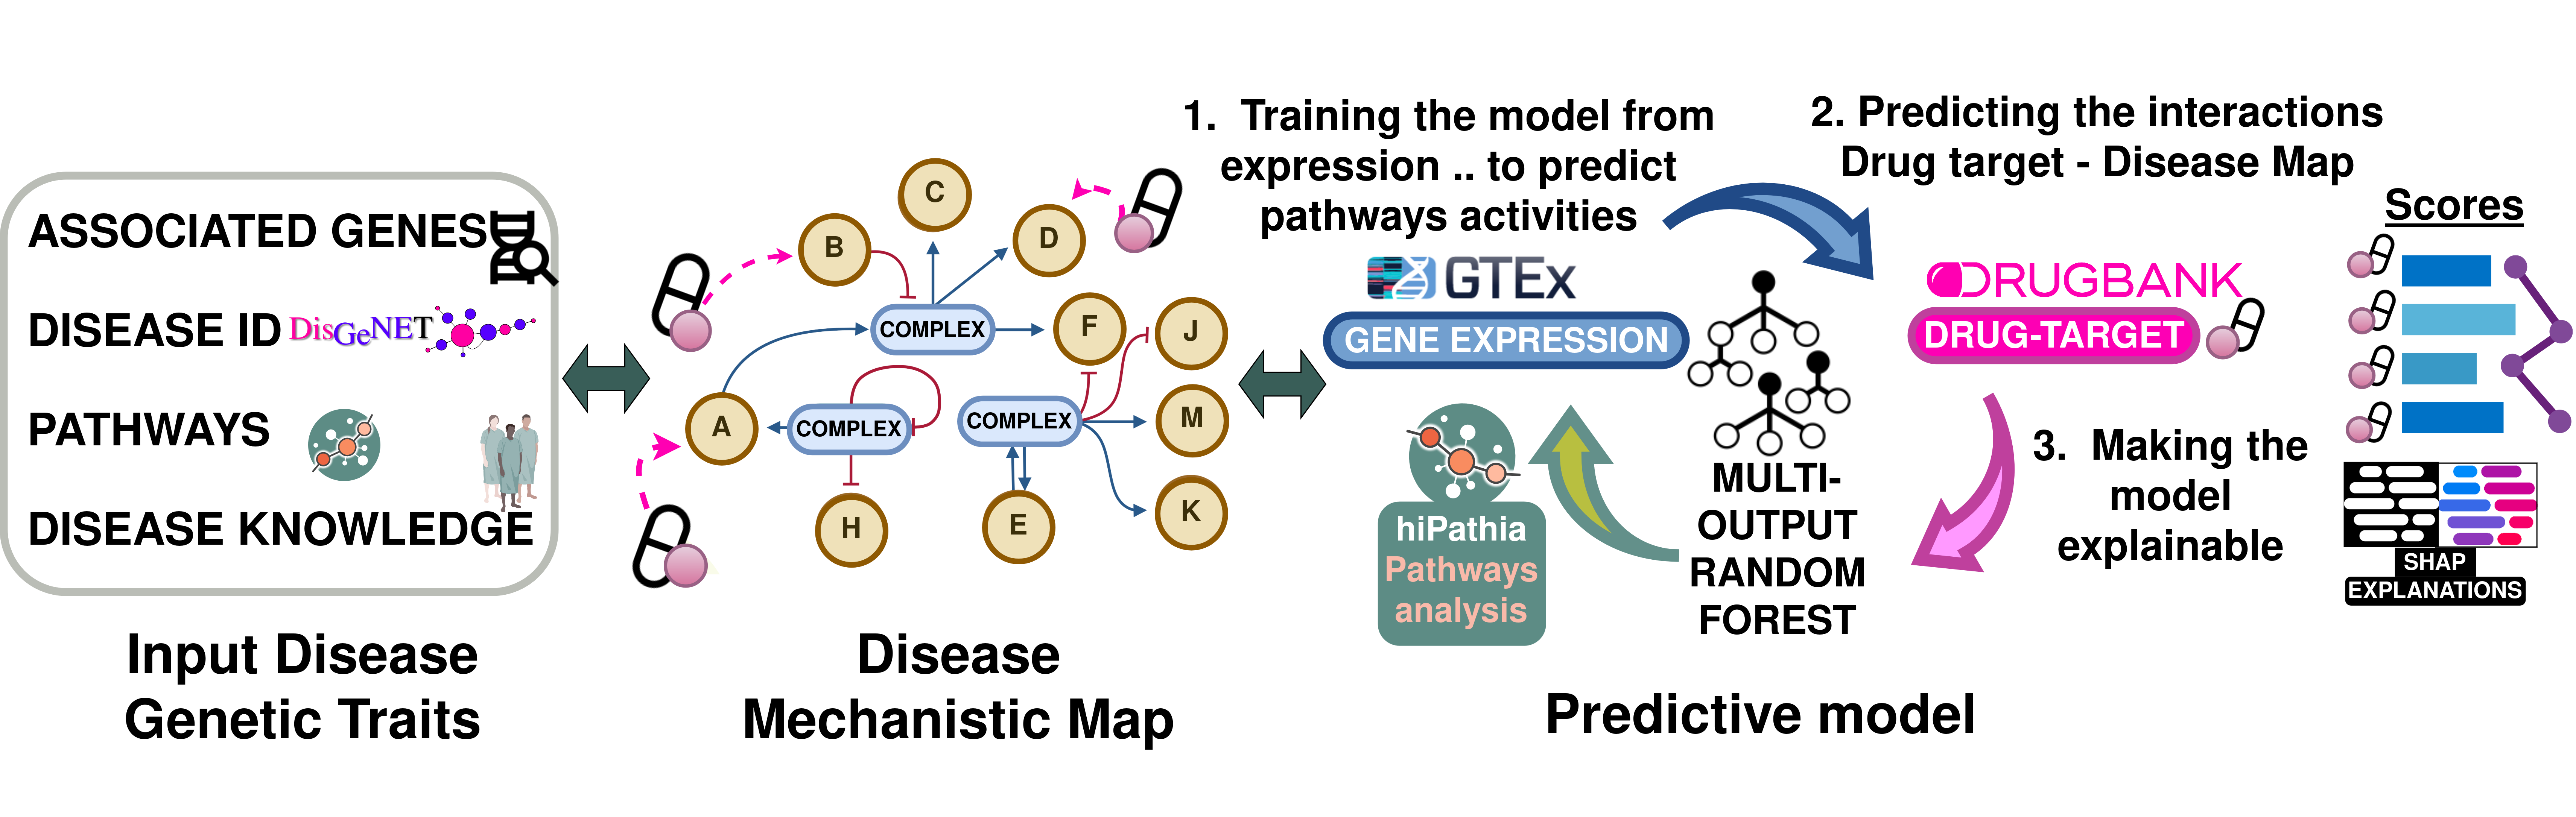
\includegraphics[width=\linewidth]{./fig/drexml_font_L.png}
            \end{tikzfigure}
        }

        % \note[rotate=8, connection=true, width = 7cm,
        % targetoffsetx=-6cm,targetoffsety=8cm
        % % roundedcorners=15, targetoffsetx=2cm
        % ]{Oh wait! A note!}
\end{columns}



\begin{columns}

    \column{0.6}
        \begin{subcolumns}
            \subcolumn{0.36}

                    \block{Métricas inteligibles}{%
                        \begin{tikzfigure}
                            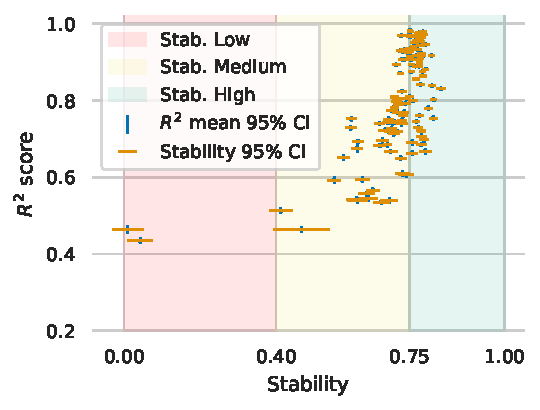
\includegraphics[width=\linewidth]{./fig/metrics.pdf}
                        \end{tikzfigure}
                    }

            \subcolumn{0.64}

                    \block{Filtrando y contextualizando}{%
                        \begin{tikzfigure}
                            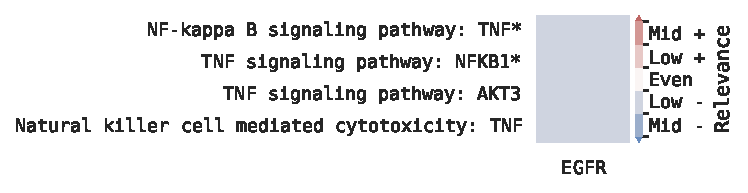
\includegraphics[width=\linewidth]{./fig/fanconi_anemia_profile_egfr.pdf}
                        \end{tikzfigure}
                    }
        
 

        \end{subcolumns}

    \block{Resultados}{
        \begin{itemize}
            \item Software Libre \colorbox{gray!10}{{\bf{pip install drexml}}}
            
            \item Fácilmente usable \colorbox{gray!10}{{\bf{drexml run disease.env}}}
            
            \item Interrogar funcionalmente a las dianas en el contexto de una enfermedad dada.
            
            \item Anemia de Fanconi
            \begin{itemize}
                \item Resultados congruentes con validaciones experimentales previas.
                \item TGF$\beta$1 y EGFR son dianas más específicas con menos efectos secundarios.
            \end{itemize}

            \item Melanoma Familiar
            \begin{itemize}
                \item Se proponen dianas que iterfieren con la vía de melanogénesis:TYR / JAK.
            \end{itemize}
            
            \item Preparada para regímenes de escasez de datos.
        \end{itemize}
    }
            
    \column{0.4}

    \block{Melanoma Familiar}{%
         \begin{tikzfigure}
             \includegraphics[width=0.92\linewidth]{./fig/heatmap_circuits_KDT_drugeff_mela.pdf}
         \end{tikzfigure}
      }


\end{columns}


\begin{columns}

    \column{0.3}
        \mtblock{2cm}{Financiación}{%
            \raisebox{-0.5\height}{
\includegraphics[width=0.45\linewidth]{./fig/ministerio.pdf}}
            \hspace{\stretch{1}}
            \raisebox{-0.5\height}{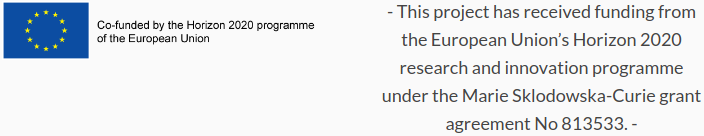
\includegraphics[width=0.45\linewidth]{./fig/mlfpm_grant.png}}
        }

    \column{0.7}
        \mtblock{2cm}{Afiliaciones del Ponente}{%
            \raisebox{-0.5\height}{
\includegraphics[width=0.24\linewidth]{./fig/andalusianplatform_color.png}}
            \hspace{\stretch{1}}
            \raisebox{-0.5\height}{
\includegraphics[width=0.25\linewidth]{./fig/fps_horizontal.png}}
            \hspace{\stretch{1}}
            \raisebox{-0.5\height}{
\includegraphics[width=0.16\linewidth]{./fig/ibis_logo.png}}
            \hspace{\stretch{1}}
            \raisebox{-0.5\height}{
\includegraphics[width=0.25\linewidth]{./fig/ciberer.png}}
        }

\end{columns}

\end{document}